\section{Microvision ShowWX+ Spezifikationen}
\label{app:projector}

\begin{table}[!ht]
\caption{Spezifikationen des Microvision ShowWX+}
\begin{center}
\vspace{-3mm}
\begin{tabular}{|l|r|}
\hline
\rowcolor{lightgray} Eigenschaft & Spezifikation \\
\hline
Auflösung 	& WVGA (848x480) \\
\hline
Seitenverhältnis & 16:9 \\
\hline
Helligkeit 	& 15 Laser-Lumen \\
\hline
Wiederholfrequenz & 60 Hz \\
\hline
Farbumfang 	& $\sim$ 200\% NTSC \\
\hline
Kontrastverhältnis 	& $>$ 5.000:1 \\
\hline
Projektionsverhältnis 	& 1:1 \\
\hline
Projektionsdistanz 	& 200 bis 2500 mm \\
\hline
Bildgröße 	& 150 bis 2500 mm \\
\hline
Verschlüsselung 	& HDCP \\
\hline
Videoeingang & HDMI (480p) \\
\hline
Gewicht 	& 122 g \\
\hline
\end{tabular}
\end{center}
\label{tab:landmarks_f1}
\end{table}

\begin{figure}[hb]
%\vspace{-30mm}
\begin{center}
		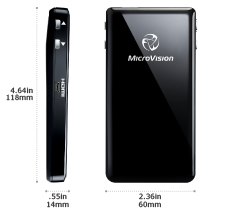
\includegraphics[scale=0.8]{measurements_showwx}
\end{center}
\vspace{-5mm}
\caption{Abmessungen des Microvision ShowWX+}
\label{fig.specs_proj}
\end{figure}

\clearpage{}

\section{Technische Spezifikationen des Arduino Nano}
\label{app:arduino}

\begin{table}[ht]
\caption{Technische Spezifikationen des Arduino Nano}
\begin{center}
\begin{tabular}{|l|r|}
\hline
\rowcolor{lightgray} \multicolumn{1}{|c|}{\textbf{Spezifikation}} & \multicolumn{1}{|c|}{\textbf{Wert}}\\
\hline
Microcontroller & Atmel ATmega328\\
\hline
Betriebsspannung & 5V\\
\hline
Eingangsspannung & 7-12V\\
\hline
Grenzen der Eingangsspannung & 6-20V\\
\hline
Digitale I/O Pins & 14\\
\hline
Analoge Eingangspins & 8\\
\hline
Gleichstrom pro I/O Pin & 40mA\\
\hline
Flash Speicher & 32KB\\
\hline
SRAM & 2KB \\
\hline
EEPROM & 1KB\\
\hline
Taktfrequenz & 16MHz\\
\hline
Länge & 45mm\\
\hline
Breite & 18mm\\
\hline
Gewicht & 5g\\
\hline
\end{tabular}
\end{center}
\label{tab:arduino}
\end{table}

\clearpage{}

\section{Technische Spezifikationen des Raspberry Pi}
\label{app:raspberry}

\begin{table}[ht]
\caption{Technische Spezifikationen des Raspberry Pi}
\begin{center}
\begin{tabular}{|l|r|}
\hline
\rowcolor{lightgray} \multicolumn{1}{|c|}{\textbf{Spezifikation}} & \multicolumn{1}{|c|}{\textbf{Wert}}\\
\hline
System-on-a-Chip & Broadcom BCM2835\\
\hline
CPU & 700MHz ARM11 ARM1176JZF-S\\
\hline
GPU & Broadcom VideoCore IV\\
\hline
Speicher & 512MB\\
\hline
USB 2.0 Ports & 2\\
\hline
Videoausgänge & Composite RCA, HDMI\\
\hline
Audioausgänge & 3,5mm Jack, HDMI\\
\hline
Low-Level Peripherie & 26 General Purpose Input/Output Pins,\\
& Serial Peripheral Bus Interface (SPI), I²C, I²S,\\
& Universal Asynchronous receiver/transmitter (UART)\\
\hline
Netzwerkschnittstelle & 10/100 wired Ethernet RJ45\\
\hline
Stromversorgung & 700mA\\
\hline
Spannungsversorgung & 5V\\
\hline
Länge & 85mm\\
\hline
Breite & 56mm\\
\hline
Höhe & 15mm\\
\hline
Gewicht & 31g\\
\hline
\end{tabular}
\end{center}
\label{tab:raspberry}
\end{table}

\clearpage{}

\section{Technische Spezifikationen des Microsoft Kinect Sensors}
\label{app:kinect}

\clearpage{}

\section{Bayes Filter}
\label{app:bayes}

\clearpage{}

\section{Konstruktionszeichnungen und Modelle}
\label{app:construction}

\clearpage{}

\section{Launchfiles}
\label{app:launchfiles}